\documentclass[journal]{IEEEtran}

\IEEEoverridecommandlockouts

% Figures and tables
\usepackage{graphicx}
\usepackage{caption}
\usepackage{subcaption}
\usepackage{booktabs}
\usepackage{multirow}
\usepackage{placeins}

% Mathematics and symbols
\usepackage{amsmath,amssymb,amsfonts}
\usepackage{bm}
\usepackage{mathtools}
\usepackage{textcomp}
\usepackage{gensymb}
\usepackage{upgreek}

% Algorithms
\usepackage{algorithm}
\usepackage{algpseudocode}

% Citations and URLs
\usepackage{cite}
\usepackage{url}

% Text, layout, and editing utilities
\usepackage{xcolor}
\usepackage{enumitem}
\usepackage{soul}
\usepackage{lipsum}
\usepackage{cuted}
\usepackage{censor}

% Preserve the document's existing roman-numeral list style.
\setlist[enumerate,1]{label=(\roman*)}

\title{NL2GPR: A Natural-Language Interface for Ground-Penetrating Radar Simulation}

\author{Vijayrathan Karthikeyan and Seyed Zekavat%
\thanks{Vijayrathan Karthikeyan and Seyed Zekavat are with Worcester Polytechnic Institute. Corresponding author: Vijayrathan Karthikeyan (email: vkarthikeyan1@wpi.edu).}}

\begin{document}

\maketitle


\begin{abstract}
Machine-learning pipelines for ground-penetrating radar (GPR) depend on large, and diverse labeled datasets that are expensive and time consuming to collect via field measurement campaigns. Generating these datasets synthetically using finite-difference time-domain (FDTD) solvers such as gprMax demands simultaneous expertise in electromagnetics, soil physics, antenna design, and solver scripting. We present NL2GPR, an agentic conversational system that turns a natural-language description of a subsurface scenario into a physically validated batch of gprMax simulations. NL2GPR pairs a single retrieval-grounded LLM agent, confined strictly to parameter elicitation, with a deterministic physics core that performs all sampling, dielectric derivation, grid design, validation, and input-file emission with no physical quantity is ever predicted by the language model. Elicited parameter ranges flow through a strict derivation chain, from Peplinski soil permittivity corners with constraint wavelength budgets to spatial discretization, Courant–Friedrichs–Lewy (CFL)-limited time stepping, and time-window selection, and are enforced by a five-tier validation hierarchy. Any violations are routed back into the ongoing dialogue, where the agent negotiates a physically admissible fix with the user in a conversational manner. The system persists sessions and simulated signals in a relational store, detects when a requested dataset is already covered by a previous run through a similarity index, and streams a live visualization of the evolving subsurface model. We verify that the system's a-priori dielectric derivations agree with gprMax's internal Peplinski model to within 0.3\%, and we outline an evaluation of extraction fidelity, physics-gate effectiveness, end-to-end generation cost, and reuse precision.
\end{abstract}

\begin{IEEEkeywords}
ground-penetrating radar, gprMax, large language models, retrieval-augmented generation, synthetic data, FDTD, soil dielectric models
\end{IEEEkeywords}


1. Introduction
   1.1 GPR for Subsurface Characterization
   1.2 The Transition Toward Intelligent GPR
   1.3 Data Requirements and Field-Data Limitations
   1.4 The Need for Synthetic GPR Data
   1.5 Physics-Based Synthetic Data Generation with gprMax
   1.6 Research Gap and Proposed Agentic Interface


2. System Overview
   2.1. Conversational Layer: Single Agent, Six-Stage Collection, RAG, and Schema-Validated Storage

   2.1.1 Stage 1: Dataset Configuration
   2.1.2. Stage 3: Buried-Target Configuration
   2.1.3. Stage 4: Waveform Configuration
   2.1.4. Stage 6: Advanced Parameters
   2.1.5. Deterministic Physics Derivation After Collection
   2.1.6. Retrieval-Augmented Geophysics Knowledge

3. Implementation
   3.1 Orchestration Runtime
   3.2 Service Layer and Persistence
   3.3 Live Subsurface Visualization
   3.4 Simulation Execution
   3.5 Deterministic Forward-Model Reuse

4. Evaluation
   4.1 E1: Extraction Fidelity
   4.2 E2: Physics-Gate Effectiveness
   4.3 E3: End-to-End Case Studies
   4.4 E4: Reuse Precision and Retrieval Quality

5. Conclusions and Future Work




\section{Introduction}
\subsection{GPR for Subsurface Characterization}

Ground Penetrating Radar (GPR) is a non-invasive geophysical sensing technique used to characterize soil subsurface medium by transmitting electromagnetic waves into the ground and analyzing the resulting reflections. Variations in the electromagnetic properties of subsurface materials, particularly dielectric permittivity and electrical conductivity, affect the propagation and reflection of the transmitted signal. Thus, the received signal includes information about the structure and composition of the soil subsurface. Because GPR can provide high-resolution measurements without excavation or physical intrusion, it has been widely adopted across several domains. In civil engineering, GPR is used for applications such as locating buried utilities and assessing pavements, bridges, tunnel linings, and other infrastructure \cite{lai2018review}. In archaeology, it enables non-destructive mapping of buried structures and archaeological features \cite{leckebusch2003ground}. In agriculture and environmental monitoring, GPR has been investigated for estimating soil water content, soil properties, and subsurface root structures \cite{liu2016ground,huisman2003measuring}. 

\subsection{The Transition Toward Intelligent GPR}

More recently, GPR research has begun moving beyond conventional signal acquisition and manual interpretation toward intelligent GPR, where machine learning (ML) models are used to extract subsurface properties directly from received radar signals and to support adaptive sensing. Intelligent GPR is specifically critical for soil subsurface assessment of a super large area such as megafarm soil moisture assessment. For example, Jahromi et al. developed an intelligent airborne GPR system in which ML models were applied to received signal features for soil moisture estimation, with the broader goal of enabling adaptive waveform selection for improved subsurface characterization \cite{jahromi2024intelligent}. Similarly, Largani et al. investigated the statistical characteristics of the soil subsurface channel for drone-borne intelligent GPR, demonstrating how soil-channel statistics can support optimal waveform design, ML-based feature extraction, and the estimation of properties such as soil moisture, permittivity, and subsurface layering \cite{largani2024soil}. Together, these developments illustrate a transition from GPR systems that primarily collect data for subsequent expert interpretation toward systems capable of learning relationships between received signals and subsurface conditions and ultimately adapting their sensing strategy based on those relationships.

\subsection{Data Requirements and Field-Data Limitations}

A major requirement for this transition is data. Machine learning models depend on sufficiently large and diverse datasets to learn the relationships between GPR responses and the underlying subsurface conditions. This requirement becomes particularly important when the objective is to build models that generalize across variations in soil texture, moisture, material properties, layer thicknesses, buried objects, antenna configurations, and transmitted waveforms. Recent reviews of ML and deep-learning applications to GPR identify the availability of large, annotated datasets as one of the primary limitations to developing robust GPR models \cite{gprMLReview}. The challenge is already evident in intelligent GPR research. For example, the airborne GPR study by Jahromi et al. \cite{} used only 24 field measurement rounds for its initial ML analysis and explicitly identified larger measurement campaigns as necessary for future development. In addition, Filardi 2023 et al. \cite{} used 50 signals for each investigated soil class when estimating soil-moisture content.

Collecting such datasets through physical GPR measurements is difficult to scale. Each measurement campaign requires radar hardware, an appropriate test site, controlled or independently measured subsurface conditions, and reliable ground-truth labels. For subsurface parameters such as moisture, layer geometry, or buried-object position, obtaining ground truth can require additional sensing equipment, manual measurements, excavation, or carefully prepared experimental environments. Repeating this process across the large number of parameter combinations required for ML training is expensive and time-consuming. Furthermore, field measurements provide limited control over environmental variability and may make it difficult to isolate the effect of individual parameters. The difficulty is therefore not simply collecting radar signals, but collecting sufficiently diverse labeled signals for which the underlying subsurface configuration is accurately known. Studies of ML-based GPR similarly identify large-scale labeled data preparation as labor-intensive and difficult, particularly when field measurements and physical ground truth are required \cite{gprMLReview}.

\subsection{The Need for Synthetic GPR Data}

These limitations create a strong need for high-quality synthetic GPR data. Numerical simulation makes it possible to generate radar measurements from controlled subsurface scenarios in which the geometry, electromagnetic properties, soil composition, moisture, target characteristics, and radar configuration are known exactly. This provides automatically available ground-truth labels and enables systematic exploration of parameter combinations that would be impractical to reproduce through field campaigns. Synthetic data have consequently become an important resource for ML-based GPR research, particularly when large labeled datasets are unavailable. However, the usefulness of synthetic data depends strongly on its physical validity and diversity. A large dataset is of limited value if the simulated scenarios violate physical constraints, cover only a narrow region of the relevant parameter space, or fail to represent the variability expected in real subsurface environments. Consequently, scalable synthetic-data generation must preserve the underlying electromagnetic and geometric constraints of the simulated GPR problem.

\subsection{Physics-Based Synthetic Data Generation with gprMax}

One of the most widely used tools for physics-based synthetic GPR data generation is gprMax. gprMax is an open-source electromagnetic simulation software specifically developed for numerical modeling of GPR. It solves Maxwell's equations using the Finite-Difference Time-Domain (FDTD) method and supports detailed specification of the computational domain, spatial discretization, electromagnetic materials, subsurface geometries, transmitting waveforms, sources, receivers, antennas, and absorbing boundary conditions \cite{warren2016gprmax}. Its ability to represent heterogeneous subsurface environments and generate GPR signals has led to its use in numerous studies as synthetic-data. For example, Largani et al.\cite{} used gprMax to generate hundreds of signals across multiple soil textural classes for statistical characterization of the soil subsurface channel.

Despite these capabilities, constructing large and diverse datasets with gprMax remains a technically demanding process. A simulation is defined through an input configuration in which the user must specify parameters such as the computational-domain dimensions, spatial discretization, simulation time window, material properties, waveform characteristics, source and receiver positions, subsurface geometry, and boundary conditions. These parameters are not independent. Spatial discretization affects numerical accuracy and computational cost, the dimensions of the domain must accommodate the modeled geometry and absorbing boundary regions, material properties determine electromagnetic propagation, and changes to layer thicknesses or object dimensions can require corresponding adjustments to the overall simulation geometry. gprMax therefore provides the underlying simulation capability, but creating reliable datasets at scale still requires users to combine knowledge of GPR, electromagnetic modeling, FDTD numerical constraints, soil subsurface property selection, soil layer selection, waveform design, antenna adoption, gprMax configuration, and programmatic parameter generation. IN addition, the user should be able to properly select how statistically diverse data should be generated. 

%\subsection{Research Gap and Proposed Agentic Interface}

This creates a significant gap between the availability of a powerful electromagnetic simulator and its operation to generate scalable data for intelligent GPR. Researchers with diverse background interested primarily in developing ML models should not need to manually translate every desired dataset variation into low-level FDTD simulation configurations while independently ensuring that the resulting scenarios remain geometrically and physically valid. 

To address this gap, this paper introduces an intelligent agentic interface for large-scale GPR synthetic-data generation using gprMax. The proposed platform provides a higher-level interface between the user's intended GPR dataset and the underlying simulation engine. This enables reduction in the expertise and manual configuration required to construct and execute diverse simulation scenarios. By combining intelligent configuration with physics-aware validation and automated simulation generation, the platform aims to lower the barrier to gprMax-based dataset creation and enable the scalable generation of physically valid synthetic GPR datasets for training and evaluating machine-learning models. Rather than requiring users to manually coordinate interdependent parameters across many input files, the proposed system manages the complete process from conversational configuration to simulation generation and structured data storage.




% \section{Introduction}

% \subsection{ Motivation:}

% Introduction 

% What is GPR? What are the applications. 
% Why people need GPR data: Application that require GPR Data. For example, GPR design or needs a preliminary studies of soil. Be specific and add citation [??]
% On example is Intelligent GPR recently emerged for which you need a huge amount of data. Refer to the team papers on Intelligent GPR; add citations. 
% Hardship of field measurements with GPR.
% gprMax has been introduced as a solution. 
% Working with gprMax is difficult as it needs diverse background.

% This paper introduces a novel chatbot capable of replacing expert domain requirement for selecting the parameters of gprMax.

% Add your contribution. 




% Subsurface assessment underpins a wide range of applications such as soil-moisture estimation, buried-object detection and infrastructure inspection. Among the available geophysical assessment tools, Ground-Penetrating Radar (GPR) offers a compelling combination of higher resolution and non-invasiveness compared to Electromagnetic Induction(EMI) and Electrical Resistivity Tomography (ERT) <CITATION>. Recent drone-borne GPR advancements <CITATION> extend this capability to large and otherwise inaccessible areas. 
% But the main issue with drone-borne or ground coupled GPR is it's expensive and time-taking. Therefore the community is increasingly coupling GPR with machine-learning (ML) models to estimate the properties of subsurface. For example: clutter removal, target detection, and full-waveform inversion.
% However, these models are data-hungry and collecting labeled real GPR data is expensive, slow, and constrained by site access. Realistic synthetic data generation is therefore the need of the hour. Open-source simulation software's like gprMax make this possible in principle through  finite-difference time-domain solving. However, in practice, accessing gprMax requires simultaneous fluency in electromagnetics, soil science, antenna and waveform design, and expertise in gprMax's own scripting interface. These barriers excludes most users. An intelligent interface that lowers this barrier and opens up the gate for large-scale physically valid datasets for ML model training is needed.

% \subsection{Relevant work:}
% Previous efforts relevant to this paper cluster into two threads, each leaving the bottleneck we target unresolved. First, the gprMax FDTD solver \cite{warren2016gprmax} supports heterogeneous soils, fractal surfaces, and arbitrary antenna/waveform definitions. gprMax also supports Python-based parameterization of simulation models,but generating diverse datasets requires users to explicitly solve the scene parameters with domain dimensions, spatial discretization, PML clearances, and geometric constraints. This becomes particularly important when varying subsurface structure, such as soil-layer thicknesses and target locations. Because changing one parameter can alter valid layer boundaries, target placement, and mesh constraints. Our framework instead treats these constraints as part of the dataset-generation process, enabling systematic variation of physically meaningful scene parameters while maintaining a consistent computational domain and discretization across samples. Therefore the resulting dataset is physically valid samples that has wider variance for the ML model to learn.

% Second, LLM-backed scientific assistants have shown value for literature search (Multi-Turn Agentic Scientific Literature Search via Workflow Induction - Jisen Li  et al) , code generation (Teaching Large Language Models to Self-Debug - Xinyun et al), and tutoring (DeepTutor: Towards Agentic Personalized Tutoring - Bingxi et al). To our knowledge, no prior system combines targeted gpr simulation parameter elicitation, physics-validated input synthesis for an FDTD solver and cross-session dataset reuse within a single conversational pipeline.

 
% \subsection{Proposed Idea:}
% We present NL2GPR, a conversational interface that opens drone-borne GPR data generation to users from across geophysics, ECE, soil science, and machine learning. Our goal is to collapse the multi-step, multi-expertise workflow that gprMax demands today, into a single guided dialogue, without sacrificing the rigor those steps require.

% A stage-orchestrated conversational layer places a single retrieval-grounded agent in charge of parameter elicitation, while a deterministic core performs all sampling, dielectric derivation, grid design, validation, and file emission. The boundary between the two is architectural, so no physical quantity ever blindly estimated by the language model.

% % We are consdiering two sxcenarios and comapring them.

% % Need a simplified figure of the structure.

% \begin{figure*}[t]
% \centering
% \includegraphics[width=\textwidth]{highlevel_arch.png}
% \caption{High level architecture}
% \label{fig:architecture}
% \end{figure*}



% % Location-based parameter elicitation deducted through extracted ISMN soil parameter stochastics

% A retrieval-augmented knowledge (RAG) base over a curated corpus of 86 GPR and soil-physics publications, together with the gprMax reference documentation, grounds every parameter-collection turn in published dielectric models, gprMax syntax, and UAV-GPR design practice rather than generic LLM priors.

% Together, these layers enable users to
% \begin{enumerate}
% \item Describe a subsurface scenario in natural language and obtain a validated batch of gprMax \texttt{.in} files.
% \item Execute batch simulations, with CPU or GPU backends, directly from the chat, with physics violations caught \emph{before} the solver runs and repaired conversationally after failure.
% \item Persist generated datasets, parameter ranges, and extracted signals in a relational store, and reuse previously simulated datasets when a new request is detected to be configuration-equivalent to an earlier one.
% \item Watch a live visualization of the configured subsurface geometry, antenna placement, and sampled realizations build up as the dialogue progresses.
% \end{enumerate}


% \subsection{Contributions:}

% The technical contributions of this paper are as follows.

% \textbf{A stage-orchestrated conversational framework with a strict agentic--deterministic boundary}: A single tool-using deep agent, operating on one persistent conversation thread, elicits all six configuration sections of a gprMax campaign (dataset scale, soil layering, buried targets, source waveform, antenna geometry, and advanced solver parameters). Stage progression is state-based rather than turn-based: the pipeline advances only when a section's schema-validated save lands in a shared section store, and users may revise any earlier section at any time. Crucially, the LLM is confined to parameter elicitation and re-elicitation; all sampling, dielectric derivation, grid design, validation, and file emission are deterministic code, so no physics ever flows through the language model.

% \textbf{A geophysics-grounded RAG knowledge base as the system's backbone}: The agent is not a bare LLM; every parameter-collection turn can consult a dedicated retrieval sub-agent over a curated corpus of 86 GPR and soil-physics publications plus the gprMax reference documentation, organized into twelve thematic categories. The corpus is ingested with layout-aware parsing (MinerU) and semantic chunking, indexed in Qdrant with hybrid dense (BGE-M3) + sparse-lexical vectors, and re-ranked with bge-reranker-v2-m3, with a confidence threshold that suppresses low-quality retrievals.

% \textbf{A physics-constrained derivation and sampling pipeline}: Pydantic-validated parameter ranges are expanded into $N$ concrete scenarios and gprMax .in files through a strict derivation chain. The soil texture and volumetric water content map to complex permittivity via gprMax's native Peplinski mixing model, worst-case wet/dry $\varepsilon_r$ corners set the wavelength budget, and spatial discretization, domain extent, CFL-limited time step, and time window follow deterministically. A five-tier validation hierarchy (schema, collection envelope, per-sample, global grid, emission) enforces $\lambda/10$ mesh resolution, CFL stability, PML clearance, domain--layer fit, Peplinski frequency-band feasibility, Ricker peak-versus-center frequency conversion, and antenna offsets. Infeasible target placements are redrawn or dropped rather than silently emitted.

% \textbf{A conversational validation-repair and regeneration loop}: Validation-gate failures are not terminal errors. Violations are injected into the ongoing agent context, where the agent explains the failed constraint, negotiates a fix with the user, and re-saves the offending section before the gate re-runs. Edits touching sampling inputs are automatically routed back through re-sampling. Post-completion edits are checked against the last successful configuration and trigger deterministic regeneration of only the affected tail of the pipeline.

% \textbf{A persistence, reuse, and access layer}: Extraction sessions, simulation runs, and extracted signals are persisted in SQL database. The conversation state is checkpointed per thread so multi-chat sessions survive restarts and resume mid-dialogue. Emitted datasets run through batch gprMax forward modeling directly from the chat, and a deterministic similarity index over completed session configurations (normalized numeric feature vectors with categorical hard filters and exact interval-IoU rescoring) detects when a requested dataset is already covered by a prior run and offers reuse in place of recomputation.



%This paper presents an agentic platform that generates a user's high-level GPR dataset through large-scale physics-based gprMax emulations. The platform addresses the gap between gprMax's low-level simulation capabilities and the requirements of researchers who need diverse, labeled datasets for machine-learning development. 

The main contribution of this work are as follows:

\begin{itemize}
\item We develop a conversational interface that collects the dataset requirements through six structured stages covering dataset size, soil layers, buried targets, waveforms, antenna configuration, and advanced simulation parameters. This process will be supported by Retrieval-Augmented Generation. Here, we gathered and created a database of all Soil, Antenna and Propagation, GPR Waveform design and GPR system-related documents and papers that contain key information for proper gprMax setting. RAG runs semantic search and provides information adopted from these documents, which reduces domain expertise required to configure a simulation campaign.


\item We separate language-based parameter collection from deterministic physics computation. The system automatically derives quantities such as material permittivity, spatial discretization, domain dimensions, antenna placement, and simulation time from the collected requirements. Physics-aware validation prevent malformed, geometrically infeasible, or numerically invalid configurations from reaching gprMax.

\item We provide an automated method for generating diverse simulation scenarios from user-defined parameter ranges. Each generated sample represents an independently varied subsurface scene, including variations in layer properties, moisture, target geometry, and target position. A common grid and computational domain are derived from the worst-case requirements of the complete dataset, ensuring numerical consistency across samples while preserving physical diversity.

\item We establish a traceable data-generation pipeline that connects each simulated GPR signal to the exact validated parameters and gprMax input configuration that produced it. The generated configurations, derived numerical parameters, artifact locations, and simulation outputs are stored in a structured database, producing labeled and reproducible datasets that can be queried and used directly for training and evaluating machine-learning models.


\end{itemize}

Together, these contributions transform gprMax from a manually configured forward simulator into a higher-level synthetic-data generation platform. The system retains the physical fidelity of gprMax while reducing manual configuration, coordinating coupled simulation parameters, enforcing dataset-wide numerical consistency, and making large-scale GPR dataset generation more accessible to machine-learning researchers.



\section{Background and Methodological Framework}


\subsection{gprMax and FDTD-Based GPR Simulation}

A GPR system consists of a transmitting antenna (Tx) and one or more receiving antennas (Rx). The transmitter radiates a short electromagnetic pulse into the ground. As the pulse propagates, changes in electromagnetic properties at soil-layer boundaries or buried objects cause part of its energy to be reflected toward the surface. The receiver records the resulting electric or magnetic field as a function of time. When the propagation velocity is known or estimated, the arrival time of a reflection provides information about the depth of the corresponding interface or target. Its amplitude and waveform are also influenced by material contrast, attenuation, target geometry, antenna configuration, and interactions with other subsurface structures.

\begin{figure}[t]
\centering
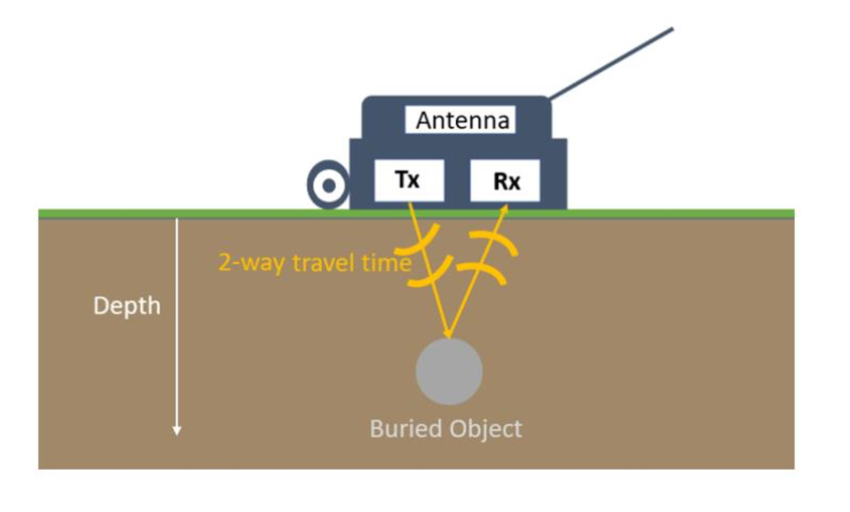
\includegraphics[width=0.90\columnwidth]{figures/txrx_representation.png}
\caption{Conceptual operation of a GPR system. The transmitter radiates an electromagnetic pulse into the subsurface, and the receiver records energy reflected by a buried object. The measured delay represents the two-way propagation time through the intervening medium.}
\label{fig:gpr_txrx}
\end{figure}

gprMax is an open-source electromagnetic simulation tool developed for numerical modeling of GPR \cite{warren2016gprmax}. It models the complete GPR forward problem. Given a computational domain, subsurface geometry, electromagnetic material properties, excitation waveform, transmitter and receiver configuration, it calculates the electromagnetic fields that would be observed over the specified simulation period. Although designed primarily for GPR, its underlying solver can represent a broader range of electromagnetic-wave propagation problems.

The simulator solves Maxwell's equations using the FDTD method. For a linear, isotropic, and electrically lossy medium, the relevant equations can be expressed as

\begin{align}
\nabla \times \mathbf{E}
&=
-\mu\frac{\partial \mathbf{H}}{\partial t}, \
\nabla \times \mathbf{H}
&=
\epsilon\frac{\partial \mathbf{E}}{\partial t}
+\sigma\mathbf{E}
+\mathbf{J}_{s},
\end{align}

where $\mathbf{E}$ and $\mathbf{H}$ are the electric and magnetic fields, $\epsilon$ is the electric permittivity, $\mu$ is the magnetic permeability, $\sigma$ is the electrical conductivity, and $\mathbf{J}_{s}$ represents the transmitting source. Permittivity primarily influences propagation velocity and wavelength. The  conductivity contributes to energy loss and signal attenuation. Spatial changes in these properties alter the electromagnetic impedance and produce the reflections measured by the receiver.

FDTD replaces the continuous spatial domain with a grid of discrete Yee cells and advances the fields through discrete time steps \cite{yee1966numerical}. Electric and magnetic-field components are arranged in space and time. At each iteration, the electric field is updated from the spatial variation of the magnetic field, followed by an update of the magnetic field from the spatial variation of the electric field. Repeating this process propagates the transmitted pulse through the computational domain and captures reflection, transmission, attenuation, and scattering.

The spatial and temporal discretizations cannot be selected independently. For a three-dimensional orthogonal grid, the time step must satisfy the Courant-Friedrichs-Lewy stability condition,

\begin{equation}
\Delta t
\leq
\frac{1}
{c_0
\sqrt{
\frac{1}{(\Delta x)^2}
+
\frac{1}{(\Delta y)^2}
+
\frac{1}{(\Delta z)^2}
}},
\end{equation}

where $\Delta x$, $\Delta y$, and $\Delta z$ are the spatial steps and $c_0$ is the speed of light in free space. The spatial resolution must also be sufficiently fine to represent the shortest wavelength and the smallest geometric feature in the model. A finer grid generally improves numerical accuracy but increases the number of cells, simulation iterations, memory consumption, and execution time.

A gprMax model is specified through a structured input file. Its essential settings define the domain dimensions, spatial discretization, and simulation time window. Material definitions assign electromagnetic properties such as relative permittivity, conductivity, relative permeability, and magnetic loss. Geometric commands place soil regions, layers, boxes, cylinders, rough surfaces, and other objects within the grid. Source commands define the excitation waveform, amplitude, center frequency, polarization, and transmitter location, while receiver commands define the locations and field components to be recorded. Perfectly Matched Layer (PML) boundaries absorb outgoing waves at the edges of the finite grid and approximate propagation through an unbounded physical environment.

During execution, gprMax advances the electromagnetic fields over the requested time window. Receiver outputs are stored in HDF5-based \texttt{.out} files and can contain the electric-field components $E_x$, $E_y$, and $E_z$ and the magnetic-field components $H_x$, $H_y$, and $H_z$. The files also preserve numerical metadata such as the spatial resolution, time step, number of iterations, and source and receiver locations. Geometry views and field snapshots can be generated separately for inspecting the model and visualizing wave propagation.

\subsection{Synthetic GPR Data Generation}

Synthetic GPR data are receiver signals generated from numerical subsurface models rather than physical measurement campaigns. Their primary advantage is that the complete scene is known. Every generated signal can be associated with exact labels describing the soil composition, moisture range, layer geometry, buried-target properties, antenna arrangement, waveform, and numerical configuration. Synthetic simulation therefore provides the control and labeling needed to construct large datasets for machine-learning development when equivalent field measurements would be expensive or very difficult to obtain.

An individual time-domain trace recorded at one transmitter-receiver configuration is commonly referred to as an A-scan. Moving the antennas along a survey line and combining a sequence of A-scans produces a B-scan. gprMax supports this operation by stepping the transmitter and receiver positions between repeated runs of the same model. Although this produces spatial variation in the measured response, the underlying soil layers, material properties, and target configuration remain unchanged. A B-scan therefore describes multiple observation positions within one physical scene rather than diversity across independent subsurface environments.

In this work, a dataset sample is defined as an independently parameterized subsurface scenario and its corresponding receiver response. Separate gprMax input models are created so that the physical scene itself can vary between samples. This enables the dataset to cover changes in soil-layer thicknesses, texture, moisture, electromagnetic properties, buried-object size, target depth, and horizontal position. The resulting collection represents many possible subsurface environments rather than repeated antenna measurements over a single fixed environment.

Soil is represented on the FDTD grid as a collection of cells, with each cell assigned constitutive properties that determine how the electromagnetic field propagates through it. Relative permittivity controls the propagation velocity and wavelength, while conductivity controls attenuation. Consequently, changing the properties assigned to individual cells or regions changes the received waveform, as illustrated in Fig.~\ref{fig:soil_cells}. Interfaces between layers produce reflections, while heterogeneous variations within a layer introduce scattering and more complex signal structure.

\begin{figure}[t]
\centering
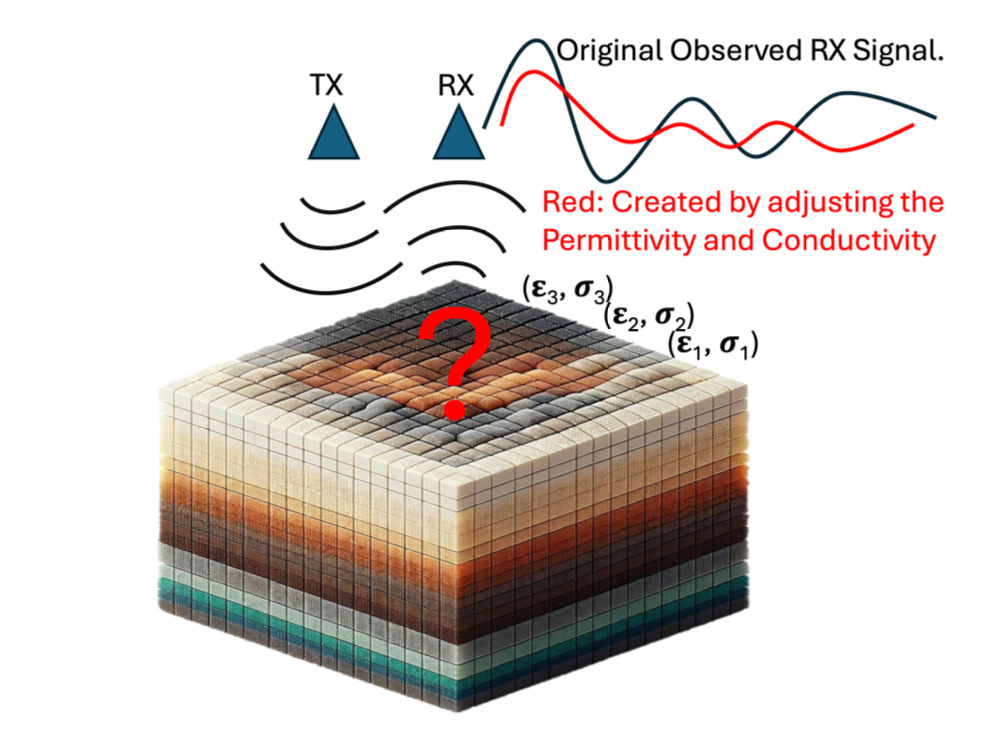
\includegraphics[width=\columnwidth]{figures/soil_cell_representation.png}
\caption{Conceptual representation of a cell-discretized subsurface model. Variations in the permittivity $\epsilon$ and conductivity $\sigma$ assigned to soil regions or individual FDTD cells change electromagnetic propagation and therefore alter the received GPR signal.}
\label{fig:soil_cells}
\end{figure}

For realistic soil generation, the platform parameterizes each layer using its sand fraction, clay fraction, volumetric water-content range, bulk density, particle density, and thickness. These physical quantities are converted into electromagnetic properties through the Peplinski dielectric soil model \cite{peplinski1995dielectric}. When combined with gprMax's heterogeneous-soil generation, the resulting layer can contain spatially distributed dielectric materials instead of behaving as a completely uniform region. This provides more realistic cell-scale variability than assigning one constant permittivity and conductivity to the entire layer \cite{giannakis2016realistic}.

Buried targets introduce another source of variation. Their geometry, dimensions, depth, horizontal offset, and material determine the shape and strength of their reflections. The current framework supports cylindrical and rectangular targets and allows their size and position to be either fixed or sampled across scenarios. A target must remain fully buried, fit within the physical domain, remain separated from the absorbing boundaries, and be large relative to the grid resolution to be represented accurately.

The waveform and antenna configuration define how each scene is observed. These parameters influence  penetration depth, resolution, and the recorded field component. 

Not all parameters should be varied independently within one dataset. In the proposed methodology, soil and target parameters provide the primary per-scenario diversity. The waveform, antenna configuration, spatial grid, and computational domain are normally shared across the generated dataset so that all samples represent a consistent acquisition setting. Separate dataset campaigns can be generated when variation in waveform or antenna configuration is required. This distinction prevents changes in numerical resolution or signal length from being confused with changes caused by the underlying subsurface physics.

Diversity is achieved by collecting physically meaningful ranges rather than one fixed configuration. Singular layer and target parameters are sampled from these ranges for each scenario. A common spatial resolution and computational domain are then derived from the most restrictive requirements across the complete sampled dataset. For example, the shortest wavelength determines an upper bound on the cell size, the smallest target feature may require a finer grid, and the deepest layer or target contributes to the required domain depth and simulation time. Using one dataset-wide numerical configuration allows the physical contents of the scene to vary while keeping the numerical basis of comparison consistent.

Parameter diversity alone does not guarantee valid simulations. Soil fractions must represent a feasible composition, volumetric water content cannot exceed the available pore volume, and the selected waveform must remain compatible with the frequency range of the dielectric model. Targets must remain buried and inside the usable domain. Sources, receivers, and objects must be separated from the PML boundaries. The grid must resolve the shortest wavelength and smallest geometric feature, the time step must satisfy the FDTD stability condition, and the time window must be sufficient for reflections from the deepest modeled region to reach the receiver.

These constraints prevent invalid random combinations from being included in the generated dataset. Physical validity in this context means that the parameters are internally consistent with the selected material models, geometry, and FDTD requirements. It does not imply that every synthetic signal exactly reproduces a particular field environment, since realism remains dependent on the assumptions used for soil, target, surface, and antenna modeling.

\subsection{High-Level System Architecture}

The proposed system places a data-generation framework around gprMax. Its architecture, shown in Fig.~\ref{fig:system_architecture}, is organized into six functional layers: the conversational interface, agent and orchestration layer, retrieval-based knowledge layer, deterministic physics and validation layer, gprMax simulation backend, and dataset and artifact layer. Together, these layers translate a user's intended dataset into validated simulation models and structured GPR signals.

\begin{figure*}[t]
\centering
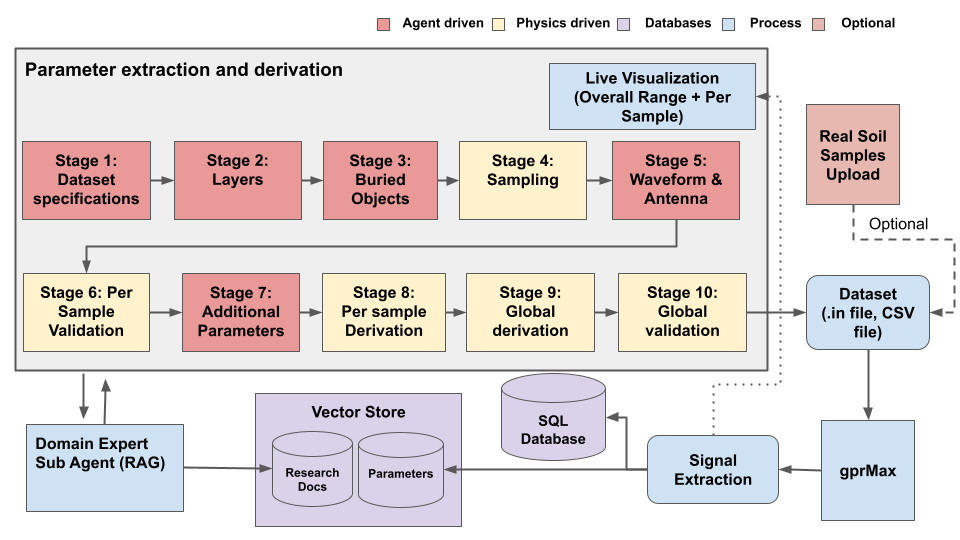
\includegraphics[width=0.96\textwidth]{figures/agent_workflow_architecture.png}
\caption{High-level architecture of the proposed synthetic GPR data-generation platform. Natural-language requirements are converted into structured parameters, supported by retrieval-based domain knowledge, processed through deterministic sampling and validation, executed using gprMax, and stored as traceable dataset artifacts.}
\label{fig:system_architecture}
\end{figure*}

The conversational interface is the primary point of interaction. It allows the user to describe a desired dataset without manually constructing gprMax input commands. The interface collects parameter ranges, presents configuration summaries, reports validation problems, and displays per-sample level visualizations. This enables the user to inspect the interpreted scene and revise parameters before expensive simulations are executed.

The agent and orchestration layer converts the conversation into structured simulation requirements. The collection agent guides the user through six conversational stages covering dataset configuration, soil layers, buried targets, waveforms, antennas, and advanced parameters. The orchestration workflow maintains the collected state, determines when a stage is complete, invokes the corresponding schema, and coordinates revisions when an earlier parameter is changed.

The processing stages shown inside the parameter-extraction and derivation region of Fig.~\ref{fig:system_architecture} represent operational phases rather than separate language-model agents. Conversational collection is followed by deterministic sampling, per-sample validation, parameter derivation, dataset-wide derivation, and global validation. This separation ensures that numerical quantities are calculated by explicit physics modules rather than generated through unconstrained language-model reasoning.

The retrieval-based knowledge layer supports the conversation with domain-specific information. It searches an indexed collection of GPR research, soil-physics literature, dielectric-model literature, and gprMax documentation. This follows the Retrieval-Augmented Generation framework, in which an external knowledge source supplements the parametric knowledge of a language model \cite{lewis2020rag}. In this architecture, retrieval is used to explain concepts and help the user make informed choices. It does not directly approve parameters or replace deterministic validation.

The physics and validation layer converts the collected requirements into realizable simulation configurations. It samples concrete soil and target scenario's then derives electromagnetic material properties establishing a common grid and domain. Then it calculates the antenna positions and simulation duration, and evaluates physical, geometric, numerical, and computational constraints. Validation occurs both at the individual-sample level and at the dataset level. Invalid dynamic samples are resampled when a feasible alternative exists, while conflicts requiring a change to the user's stated requirements are returned through the conversational interface.

After validation, the gprMax backend generates one input file for each retained scenario and executes the corresponding FDTD simulation. gprMax produces the receiver signals and simulation metadata, while the surrounding workflow manages model identifiers, file locations, execution status, and failures. This preserves gprMax as the authoritative electromagnetic solver while automating the configuration and execution processes around it.

Finally, the dataset and artifact layer extracts the required field components from the gprMax output files and associates them with the exact parameters that produced them. Generated artifacts include gprMax input files, sampled-parameter manifests, derived global configurations, receiver-signal arrays, visualization files, and database records. Structured storage makes each signal traceable to its soil, target, waveform, antenna, grid, and domain configuration. The resulting dataset can therefore be filtered, reproduced, and used directly in downstream machine-learning experiments.


Overall, the architecture assigns different responsibilities to the language model and the numerical workflow. The conversational and retrieval layers provide accessibility and domain guidance. The orchestration layer maintains state and controls execution order. The physics and validation modules enforce simulation correctness, and gprMax performs the electromagnetic calculation. This division allows the platform to simplify large-scale GPR dataset generation without transferring numerical control to the language model.



\section{System Overview}

% 2.1 gprMax and its components along with two figures

% 2.2 diverse data generation and labeling one figure

% 2.3 chatbot system architecture one figure 

\subsection{ Conversational Layer: Single Agent, Six-Stage Collection, RAG, and Schema-Validated Storage}

The conversational layer serves as the interface between the user's intended GPR dataset and the lower-level parameters required to construct physically valid gprMax simulations. Rather than requiring the user to directly specify a complete gprMax input configuration, the platform uses a single stateful conversational agent to progressively construct the simulation specification. The agent operates over one persistent conversation thread and collects the required information through six stages: dataset configuration, soil layer configuration, buried-target configuration, waveform configuration, antenna configuration, and advanced parameters. The same agent is retained throughout the complete interaction, allowing information introduced earlier in the conversation to remain available when later parameters are collected or when an earlier choice must be revised.

This architecture deliberately separates language-based parameter collection from deterministic physics computation. The agent interprets user intent, explains parameters, asks for missing information, and converts the resulting values into structured representations. It does not calculate the FDTD grid, electromagnetic material properties, propagation wavelengths, simulation domain, or simulation time window itself. These quantities are derived by deterministic physics modules after the required user parameters become available. This separation reduces the dependence of simulation correctness on unconstrained LLM reasoning. The agent determines *what the user wants to simulate*, while the physics and validation layers determine *whether that configuration is physically and numerically realizable*.

At the beginning of each collection stage, the orchestration layer injects a stage-specific instruction containing the parameters that must be collected, relevant physical constraints, default values, and the JSON schema that the final output must satisfy. The agent then collects the parameters through natural conversation. Once sufficient information has been obtained, the complete section is submitted through a schema-validation tool. A stage is considered complete only after the corresponding structured object has passed validation and has been stored. Because the same agent and conversation thread are used across all six stages, a user can also revise a previously specified quantity. For example, the user may change a soil moisture range while discussing the antenna configuration. The agent retrieves the previously stored soil section, modifies the requested values, and stores the complete updated section again. Changes to parameters that affect sample generation automatically invalidate the previously sampled parameter sets and cause them to be regenerated before the downstream physics calculations are repeated.

\subsubsection{Stage 1: Dataset configuration}

The first stage establishes the global policies that control how the dataset will be generated. The agent collects the requested number of samples and a model name together with the parameters that determine the numerical resolution and boundary policy of the eventual FDTD model. These include the number of Perfectly Matched Layer (PML) cells, the number of additional buffer cells, the desired number of cells per wavelength, the number of materials used by the gprMax Peplinski soil representation, and the frequency factor used to determine the highest significant frequency represented by the grid.

The number of samples \(N_s\) represents the number of independent gprMax input models to generate, rather than the number of temporal samples in a single radar trace. Each generated input file corresponds to one sampled subsurface configuration. The current implementation fixes the simulations to two dimensions and manages the output directory internally, so these deployment-level quantities are not exposed as user-selectable parameters.

The parameter \(N_{\lambda}\), determines the target FDTD spatial resolution. FDTD solves Maxwell's equations on a discrete Yee grid \cite{yee1966numerical}, and the spatial step must therefore be sufficiently smaller than the shortest electromagnetic wavelength represented in the simulation. The platform later derives the minimum wavelength as

$$
\lambda_{\min} =
\frac{c_0}
{f_{\mathrm{high}}\sqrt{\epsilon_{r,\max}}},
$$

where \(c_0\) is the speed of light in free space, \(f_{\mathrm{high}}\) is the highest significant frequency considered in the waveform, and \(\epsilon_{r,\max}\) is the largest relative permittivity encountered across the generated soil configurations. The initial wavelength-based cell size is then

$$
\Delta_{\lambda} =
\frac{\lambda_{\min}}{N_{\lambda}}.
$$

The agent does not calculate either quantity during collection because the necessary soil permittivity is not yet known. Instead, it collects the resolution policy and allows the deterministic derivation stage to calculate the actual grid after the soil and waveform parameters have been established.

The PML and buffer parameters serve a different purpose. PMLs are absorbing boundaries used to approximate an open electromagnetic domain and suppress artificial reflections from the edges of the finite simulation space. In the two-dimensional implementation, PML cells are applied only to the in-plane boundaries because the out-of-plane dimension consists of a single computational cell. The additional buffer separates physical objects and sources from the absorbing region. These quantities later contribute to the domain dimensions and source/object clearance conditions.

Importantly, quantities such as the final cell size, domain width, soil depth, source height, and simulation time window are deliberately *not* collected from the user. They are consequences of the requested physics and are therefore derived automatically downstream.

\subsubsection{Stage 2: Soil layer configuration}

The second stage describes the subsurface medium. The user first specifies the number of layers and then provides a range of possible properties for each layer. These properties include layer thickness, sand fraction, clay fraction, volumetric water content, bulk density, and particle density. Ranges are collected instead of individual values because the objective is to generate a dataset spanning a controlled parameter space rather than to create a single fixed GPR scene.

Only sand and clay fractions are directly collected. The silt fraction is derived through texture closure as

$$
S_{\mathrm{silt}}
=
100 -
S_{\mathrm{sand}} -
S_{\mathrm{clay}}.
$$

Consequently,

$$
S_{\mathrm{sand}}
+
S_{\mathrm{silt}}
+
S_{\mathrm{clay}}
=
100.
$$

This prevents the three soil fractions from being independently specified in a way that produces an impossible soil composition.

The densities also provide a physical constraint on the allowable soil moisture. Soil porosity is computed from the bulk density \(\rho_b\) and particle density \(\rho_p\) as

$$
\phi = 1-\frac{\rho_b}{\rho_p}.
$$

Physically, \(\rho_b < \rho_p\) must hold for the material to contain pore space. In addition, the volumetric water content \(\theta_v\) cannot exceed the available pore volume,

$$
\theta_v \leq \phi.
$$

Because the conversational stage collects ranges rather than a single density pair, an initial feasibility check uses the loosest achievable soil configuration:

$$
\phi_{\max}
=
1-
\frac{\rho_{b,\min}}
{\rho_{p,\max}}.
$$

The upper moisture bound must therefore satisfy

$$
\theta_{v,\max} \leq \phi_{\max}.
$$

This check prevents the agent from accepting a moisture range that could not be supported by any soil realization within the specified density ranges.

The current platform uses the Peplinski dielectric soil model, which relates soil texture, density, volumetric water content, and frequency to the electromagnetic response of the soil \cite{peplinski1995dielectric}. The model was developed for the 0.3 to 1.3 GHz range. The implementation therefore carries the Peplinski calibration limits into the collection and validation process, including constraints on moisture and warnings when sampled sand, silt, or clay compositions fall outside the calibration region.

After the layer ranges are collected, the deterministic sampler generates \(N_s\) concrete subsurface realizations. Thickness, sand fraction, clay fraction, bulk density, and particle density are sampled from their respective ranges. Silt is then calculated using the texture-closure equation above. Each sampled realization is checked again because a set of individually valid ranges can still produce an invalid combination. For example, a particular random draw may produce a bulk and particle density pair whose porosity is lower than the requested moisture bound. Such a draw is rejected and resampled rather than being propagated into the dataset.

The moisture interval itself is retained as a band rather than reduced to a single random value. This is required because gprMax's `\#soil\_peplinski` implementation constructs a set of dielectric materials spanning a volumetric water-content interval. Maintaining the moisture band therefore preserves the heterogeneous soil representation that will later be constructed by gprMax.

\subsubsection{Stage 3: Buried-target configuration}

The third stage allows the user to introduce buried objects. The stage is optional, so datasets containing only layered soils can be created without specifying a target. In the current two-dimensional implementation, the supported target geometries are cylinders and rectangular boxes. Objects are represented as perfect electric conductors (PECs), while their position and size can vary across the dataset.

The user specifies the horizontal target position as an offset from the survey center and the vertical position as the depth of the object's center below the ground surface. Using a center-relative coordinate system is important because the computational domain has not yet been derived at this stage. Target specifications are therefore independent of the eventual absolute domain coordinates.

For a cylindrical target, the collected range contains its center offset, center depth, and radius. For a box, the corresponding quantities are center offset, center depth, width, and height. A target may be made static by setting the minimum and maximum of every range to the same value. Otherwise, its geometry and position are sampled independently for each generated scene.

The first physical requirement is that the object remain completely buried. For a cylinder with center depth \(d\) and radius \(r\),

$$
d \geq r,
$$

while a box of height \(h\) requires

$$
d \geq \frac{h}{2}.
$$

Target dimensions also affect the FDTD resolution. A target that is much smaller than the electromagnetic wavelength may still need to be explicitly resolved geometrically. The platform therefore requires the smallest target feature to occupy at least ten grid cells. If \(d_{\min}^{\mathrm{feature}}\) denotes the smallest geometric feature observed across all sampled targets, the final spatial step is tightened according to

$$
\Delta
=
\min
\left(
\frac{\lambda_{\min}}{N_{\lambda}},
\frac{d_{\min}^{\mathrm{feature}}}{10}
\right).
$$

For a cylinder, the feature is its diameter; for a box, it is the smaller of its width and height. Consequently, a very small target can force a substantially finer grid even when the wavelength criterion would permit a coarser one.

Target ranges are sampled together with the layer ranges before waveform collection continues. At this point only domain-independent quantities are generated. Absolute target placement is postponed until the global domain has been derived. This ordering allows one common grid to be constructed from the worst-case target size, extent, and depth across the entire dataset.

\subsubsection{Stage 4: Waveform configuration}

The fourth stage specifies the electromagnetic excitation. The agent collects the waveform type, amplitude, center frequency, waveform identifier, and optional source start and end times. gprMax supports multiple excitation functions, including Ricker and Gaussian-family waveforms, while the default configuration in the platform uses a Ricker wavelet.

Frequency is particularly important because it couples the transmitted waveform to both the soil dielectric model and the numerical resolution. For the Ricker waveform, the platform derives the effective frequency band using the frequency relationships described by Wang \cite{wang2015frequencies}. If \(f_p\) is the Ricker peak frequency, the implemented lower and upper band limits are

$$
f_{\min}=0.481623f_p,
$$

and

$$
f_{\max}=1.636567f_p.
$$

The bandwidth is therefore

$$
B=f_{\max}-f_{\min}.
$$

Because the Peplinski soil model is used throughout the generated dataset, the entire derived waveform band must fall within its 0.3 to 1.3 GHz validity interval,

$$
f_{\min}\geq 0.3\;\mathrm{GHz},
\qquad
f_{\max}\leq 1.3\;\mathrm{GHz}.
$$

Checking only the user-provided center frequency would be insufficient because a center frequency inside the interval could still produce spectral content extending beyond the model's validity range.

A second frequency quantity is used for FDTD resolution. If \(\alpha\) is the configured high-frequency factor and \(f_c\) is the collected center frequency, the platform uses

$$
f_{\mathrm{high}}=\alpha f_c
$$

when determining the shortest wavelength and therefore the cell size. This is intentionally separate from the Peplinski band-validity calculation. The first quantity controls numerical resolution, whereas the second determines whether the dielectric model is being used inside its calibrated frequency range.

\subsubsection{Stage 5: Antenna configuration}

The fifth stage configures the transmitter and receiver geometry. The supported source types include a Hertzian dipole, voltage source, and transmission line. The agent collects the source type, polarization axis, transmitter-receiver separation, receiver-height policy, and optionally the source height or a receiver array.

For voltage-source and transmission-line configurations, the internal resistance must satisfy

$$
0 < R < Z_0,
$$

where

$$
Z_0 \approx 376.73\ \Omega
$$

is the impedance of free space. A Hertzian dipole does not require this resistance parameter.

The transmitter-receiver offset is used after the global domain width \(L_x\) has been established. The pair is centered around the survey midpoint:

$$
x_{\mathrm{Tx}}
=
\frac{L_x}{2}
-
\frac{d_{\mathrm{TR}}}{2},
$$

$$
x_{\mathrm{Rx}}
=
\frac{L_x}{2}
+
\frac{d_{\mathrm{TR}}}{2},
$$

where \(d_{\mathrm{TR}}\) is the requested transmitter-receiver separation.

Source height may be explicitly provided by the user. If it is omitted, the system derives it from the largest relevant wavelength,

$$
h_s = \frac{\lambda_{\max}}{2},
$$

where

$$
\lambda_{\max}
=
\frac{c_0}
{f_{\min}\sqrt{\epsilon_{r,\min}}}.
$$

Free space is included when computing \(\epsilon_{r,\min}\), since the antenna is located in the air region above the soil and air may therefore produce the largest wavelength in the model.

Once the waveform and antenna stages are complete, the first dataset-wide validation gate is executed. The waveform is checked against the Peplinski frequency window and the antenna configuration is checked for valid polarization, resistance, and source timing. Failure does not terminate the workflow. Instead, the validation error is injected back into the same conversational thread. The agent explains the conflicting parameter to the user, obtains a corrected value, rewrites the affected schema section, and the deterministic validation is executed again.

\subsubsection{Stage 6: Advanced parameters}

The final collection stage contains optional simulation features that are not required for a basic dataset. These currently include surface roughness and field snapshots.

Surface roughness is parameterized through a fractal dimension, directional weights, roughness amplitude, an optional water layer, and an optional random seed. When a water layer is requested, its depth is constrained relative to the surface roughness amplitude to maintain a meaningful geometry. The random seed allows the stochastic rough surface to be reproduced when required.

Snapshots specify the simulation time at which the electromagnetic field should be exported, together with an output filename and, optionally, a spatial extent and resolution. These parameters are kept separate from the core soil, waveform, and antenna specification because they affect diagnostic output rather than the fundamental subsurface parameter space. The complete advanced stage may also be explicitly skipped, in which case an empty but schema-valid configuration is stored.

\subsubsection{Deterministic physics derivation after collection}

After the six conversational sections have been collected, the system has sufficient information to derive a common numerical model for the complete dataset. The derivation is performed deterministically rather than by the language model.

First, the platform computes the electromagnetic properties of every sampled soil layer using the gprMax implementation of the Peplinski model itself, rather than implementing an independent approximation. For each sampled layer, the sand fraction, clay fraction, bulk density, particle density, and moisture band are passed to gprMax's `PeplinskiSoil` routine. gprMax constructs the corresponding Debye materials over the moisture interval. The frequency-dependent real permittivity is then evaluated at the operating frequency.

Two extrema are retained across every layer of every sampled scene:

$$
\epsilon_{r,\max}
=
\max_{i,j}
\epsilon_{r,i,j}^{\mathrm{wet}},
$$

and

$$
\epsilon_{r,\min}
=
\min_{i,j}
\epsilon_{r,i,j}^{\mathrm{dry}},
$$

where \(i\) indexes samples and \(j\) indexes layers. The wettest condition produces the largest permittivity and therefore the shortest wavelength, making \(\epsilon_{r,\max}\) the conservative value for spatial resolution. Conversely, the driest condition produces a larger wavelength and contributes to the required spatial extent. Using gprMax's own material implementation ensures that the dielectric properties used to size the grid are consistent with those eventually used by the forward solver \cite{warren2016gprmax}.

The global soil depth must accommodate both the largest possible layer stack and the required radar range. If

$$
D_{\mathrm{layers}}
=
\sum_j t_{j,\max}
$$

is the deepest possible layered profile, the bandwidth-limited range term used by the system is

$$
D_{\mathrm{range}}
=
\frac{c_0}
{2B\sqrt{\epsilon_{r,\max}}}.
$$

The initial soil depth is therefore

$$
D =
\max
\left(
D_{\mathrm{layers}},
D_{\mathrm{range}}
\right),
$$

and it is increased further when necessary to accommodate the deepest sampled buried target while maintaining the required separation from the PML.

The final horizontal and vertical domain dimensions are then constructed from the wavelength, transmitter-receiver spacing, target extents, soil depth, source height, PML thickness, and safety buffers. The dimensions are rounded upward to integer multiples of \(\Delta\), ensuring that every generated model lies on an integer Yee grid. Most importantly, this derivation is performed once for the complete dataset, using the worst-case parameter values across all sampled scenes. Every generated sample therefore uses the same grid spacing and overall numerical domain. Only the physical contents of that domain vary from sample to sample. This consistency is valuable for downstream machine-learning applications because differences between samples originate from the sampled physical parameters rather than unintended changes in numerical discretization.

For a uniform grid, the platform computes the FDTD time step according to the Courant stability condition. For a \(D\)-dimensional simulation,

$$
\Delta t
=
\frac{\Delta}
{c_0\sqrt{D}}.
$$

For the current two-dimensional implementation, \(D=2\). The simulation time window is then selected to allow a transmitted pulse to travel to the deepest relevant region and return to the receiver. Using the slowest propagation velocity,

$$
v_{\min}
=
\frac{c_0}
{\sqrt{\epsilon_{r,\max}}},
$$

the implemented time window is

$$
T =
\frac{2(h_s+D)}{v_{\min}}
+
\frac{2}{f_p}.
$$

The first term covers two-way propagation from the antenna to the deepest modeled region, while the second provides an additional pulse-duration margin.

The resulting global configuration is subjected to a second validation gate. Grid resolution, domain alignment, Debye stability, PML dimensions, transmitter and receiver clearance, source height, layer-stack depth, time-window sufficiency, static-target placement, memory requirements, and estimated iteration count are evaluated in a cascade. Fundamental grid errors are resolved before dependent placement checks are attempted. If a hard validation fails, the error is returned to the same conversational agent, which works with the user to modify the responsible collected parameter and then reruns the affected sampling and derivation stages.

Dynamic buried targets receive one final per-sample placement check against the fixed global grid. If a sampled target violates the PML clearance, burial, domain, or ten-cell resolution requirements, the target is redrawn within the valid geometric envelope. If no feasible placement can be found after a bounded number of attempts, the entire sample is removed rather than emitting a partially specified or physically invalid scene. Static targets are never repositioned automatically because their fixed location represents an explicit user choice; invalid static placements instead return to the user for correction.

\subsubsection{Retrieval-Augmented Geophysics Knowledge}

Although the platform is designed to remove the need for detailed gprMax expertise, many parameters still represent specialized concepts in electromagnetics, soil physics, and GPR. A user may reasonably ask questions such as what volumetric water content represents, why PML cells are necessary, how a Ricker waveform differs from a Gaussian waveform, or what soil texture range should be used for a particular experiment. Answering these questions exclusively from the language model's parametric knowledge would weaken the grounding of the interface.

To address this problem, the conversational layer incorporates Retrieval-Augmented Generation (RAG). RAG combines the parametric knowledge of a language model with externally retrieved information, allowing generation to be conditioned on relevant passages from a non-parametric knowledge source \cite{lewis2020rag}. In the proposed system, the external knowledge base contains GPR research material, soil and dielectric-model references, and gprMax documentation.

During knowledge-base construction, technical documents are parsed and divided into semantically coherent chunks. PDF documents are processed using layout-aware parsing that preserves technical content such as equations and tables, while text and Markdown sources are ingested directly. Each chunk is associated with metadata such as topic, document type, publication year, author, title, and source.

The retrieval index is implemented in Qdrant using both dense and sparse representations generated with BGE-M3. BGE-M3 supports dense and sparse lexical retrieval within a common embedding model \cite{chen2024bgem3}. For a user query \(q\), the system generates both representations and independently retrieves dense and sparse candidate sets. Their rankings are combined using Reciprocal Rank Fusion (RRF) \cite{cormack2009rrf}. For a document \(d\), RRF can be written as

$$
\operatorname{RRF}(d)
=
\sum_{r\in R}
\frac{1}{k+r(d)},
$$

where \(R\) is the set of input rankings, \(r(d)\) is the position of document \(d\) in ranking \(r\), and \(k\) is a rank-stabilizing constant. Combining dense semantic matching with sparse lexical matching is useful in the GPR domain because queries may contain both conceptual language and highly specific terminology such as `\#soil\_peplinski`, PML, FDTD, or dielectric-model parameter names.

The fused candidates are subsequently passed through a BGE cross-encoder reranker. The reranker evaluates the query and candidate passage jointly and produces a relevance score. The current retrieval pipeline first obtains candidate results from both dense and sparse search, fuses them with RRF, reranks the combined candidates, and returns the highest-ranked passages above a relevance threshold.

RAG is integrated into the agent as an auxiliary knowledge agent rather than as another parameter-collection agent. The single conversational agent remains responsible for all six simulation sections and is the only agent that modifies the parameter store. When the user asks a domain-knowledge question, the collection agent delegates that question to the knowledge component. The knowledge agent searches the indexed corpus, synthesizes the retrieved information, and returns the explanation to the main conversational agent. The main agent then resumes the same stage without losing the state of the parameter-collection process. If no sufficiently relevant material is retrieved, the knowledge component may fall back to general domain knowledge, but the response is explicitly distinguished from one grounded in retrieved documents.

This design gives RAG a supporting rather than authoritative role. Retrieved material helps the user understand parameters and make informed decisions, but retrieval cannot bypass the schema or deterministic physics validators. For example, RAG may explain what a realistic soil bulk density means, but the final value must still satisfy the layer schema and the derived porosity constraints. Similarly, it may explain the role of center frequency, but the waveform still has to pass the deterministic Peplinski frequency gate. This preserves the usefulness of an intelligent conversational interface without treating language-model output as a substitute for numerical validation.

\subsubsection{Schema-validated state and dataset storage}
A central requirement of the conversational architecture is that natural-language interaction must ultimately produce structured and reproducible simulation data. The platform therefore places a schema-validation boundary between the conversational agent and the downstream simulation pipeline.

Each of the six stages is represented by a dedicated Pydantic schema. When the agent attempts to save a section, the generated JSON is parsed and validated before it can enter the parameter store. Required fields, data types, range ordering, enumeration constraints, and local physical invariants are checked at this boundary. For example, a layer cannot be stored if a minimum value exceeds its corresponding maximum, if the declared number of layers differs from the number supplied, or if the requested moisture envelope cannot fit within the maximum achievable porosity. Likewise, an antenna requiring an internal resistance cannot be stored without a resistance satisfying its permitted range.

Schema validity and physics validity are deliberately treated as different levels of assurance. The schema determines whether a parameter section is structurally and locally consistent. The deterministic sampling and global validation stages subsequently determine whether combinations of those sections produce a physically and numerically valid simulation. This layered design prevents the schema from becoming an overly complex substitute for the physics engine while also preventing malformed LLM output from reaching that engine.

The validated sections are maintained as structured state throughout the conversation. The complete state includes the original dataset configuration and parameter ranges, while intermediate manifests record the concrete parameters sampled for every generated scene and the globally derived FDTD configuration. Once input-file generation is complete, the finalized dataset is persisted in PostgreSQL.

Storage is performed at two levels. A session-level record preserves the original user-specified ranges, waveform and antenna configuration, advanced parameters, global derivation, artifact locations, and dataset-generation status. In parallel, each successfully emitted simulation receives its own database row containing the concrete sampled soil layers, buried-target geometry, waveform and antenna parameters, FDTD grid information, and generated input-file path. After the forward gprMax simulation is executed, the resulting electromagnetic field components can be attached to the same simulation record.

This association between validated input parameters and corresponding simulated signals is important for machine-learning dataset quality. Each signal is traceable to the exact physical configuration that generated it, rather than to an unstructured conversational description. The database can therefore be filtered or queried by soil composition, moisture, target characteristics, antenna parameters, or other simulation attributes when constructing downstream training sets. It also prevents an important class of data-integrity errors in which a generated signal becomes detached from the parameter values that produced it.

The same integrity principle is applied when the user edits a completed configuration. Changes to sampling-dependent sections invalidate the old sampled realizations, causing the affected deterministic stages to run again. When the regenerated dataset is finalized, the previous per-sample database records for that session are replaced rather than retained alongside the new samples. Consequently, stale parameter records are not silently associated with newly generated input files or simulation outputs.

Together, the single-agent conversational workflow, retrieval-grounded knowledge support, deterministic physics layer, and schema-validated storage form a controlled translation path from natural-language intent to machine-learning-ready GPR data. The language model provides flexibility at the user interface, while the simulation state, physical derivations, validation gates, and database representation remain explicit and structured. This division of responsibility is what allows the platform to simplify interaction with gprMax without transferring control of numerical correctness to the language model.



% \section{System Architecture}
% \label{sec:architecture}


% \begin{figure*}[t]
% \centering
% \includegraphics[width=\textwidth]{NL2GPR_Architecture_v2.png}
% \caption{NL2GPR architecture. A single retrieval-grounded agent (top) elicits parameter ranges into a schema-validated section store; the deterministic core (bottom) consumes the store to sample, derive, validate, and emit gprMax models. The dashed boundary separates the agentic layer from the deterministic core: no physics crosses it in the LLM direction.}
% \label{fig:architecture}
% \end{figure*}

% \subsection{Design Principle: a Hard Agentic--Deterministic Boundary}
% \label{sec:boundary}

% The central design decision in NL2GPR is a strict, architecturally enforced separation of concerns. The \emph{agentic layer} performs parameter extraction and re-elicitation only: it converses with the user, consults the retrieval corpus, and writes structured parameter ranges into a typed store. The \emph{deterministic core} performs sampling, dielectric derivation, grid design, validation, input-file emission, and solver execution.

% This boundary is motivated by a failure mode we observed in an earlier design. A language model asked to fix a numerical error can silently paper over a genuine physics violation (e.g., relaxing a mesh criterion to make a run succeed), corrupting every sample in the emitted dataset. In the present architecture the LLM is only consulted for \emph{human} decisions such as infeasible soil texture, an out-of-band frequency, while derivable constraints are enforced by deterministic physics function and double checked by validators \emph{before} any simulation starts. Consequently, identical parameter ranges always produce identical derivations. Every derived quantity is traceable to a published formula, and the correctness of the physics is independent of the LLM's competence.

% \subsection{Stage-Based Single Agent vs Shared Parameter Multi Agent Parameter Elicitation}
% \label{sec:agent}

% An earlier prototype of NL2GPR used six isolated per-section agents coordinating through a shared parameter server. This design suffered from context fragmentation. Each agent saw only its own slice of the conversation, so cross-section edits required explicit patch machinery. NL2GPR therefore uses \emph{one} tool-using deep agent on \emph{one} persistent conversation thread, retaining the full dialogue history across all stages and both remediation flows.

% The agent collects six configuration sections in pipeline order: dataset configuration (sample count, dimensionality, output naming), soil layers, buried-target ranges, source waveform, antenna geometry, and optional advanced parameters (surface roughness, field snapshots). Three mechanisms structure the collection:

% \textbf{Schema-validated section store.} The agent has exactly two state tools: \texttt{save\_section}, which validates a complete JSON payload against the section's Pydantic schema and stores it only if valid. An invalid payload is rejected with a machine-readable error, the agent must resolve with the user, and nothing is stored. The other tool is \texttt{get\_section}, which reads a section back. There is no partial-update path: editing a section means re-saving it in full, which keeps the store's invariants simple and makes every write re-validate the whole section. A payload can be schema-valid yet incomplete (missing essential fields). In that case, the tool stores it but flags it, and the stage does not complete.

% \textbf{State-based stage progression.} The orchestrator injects a system prompt message to each stage. The section's are informed about the grouping of parameters and JSON schema. Progression is  decided by inspecting the store, never by parsing the agent's prose or scraping its tool calls, which makes the pipeline robust to conversational variation.

% \textbf{Staleness-tracked cross-section edits.} Because the whole dialogue lives on one thread, the user may revise any earlier section at any time. Sections that are inputs to the sampler (dataset configuration, layers, target ranges) are marked as re-sample triggers. The sampling stage snapshots its inputs, and a conditional edge re-runs sampling before the derivation chain, whenever the snapshot no longer matches the store. An edit therefore can never leave downstream artifacts silently inconsistent with the configuration that is on record.

% \subsection{Retrieval-Grounded Knowledge}
% \label{sec:rag}

% Domain questions are delegated to a dedicated retrieval sub-agent over a curated corpus of 86 GPR and soil-physics publications plus the gprMax reference documentation, organized into twelve \emph{thematic categories} (solver documentation, FDTD numerics, antenna modeling, soil dielectric models, UAV-GPR platforms, waveform design, and others). Documents are parsed with layout-aware OCR and split by semantic chunking (embedding-distance percentile breakpoints). Then we index the vectors in Qdrant vector database with \emph{dense embeddings} vectors (BGE-M3) and sparse lexical weights \cite{chen2024bge}. Queries retrieve on both channels, candidates are re-ranked with a cross-encoder (\texttt{bge-reranker-v2-m3}), and a confidence threshold suppresses low-quality retrievals, so the agent prefers asking the user over quoting a marginal passage. This way the sub-agent grounds the \emph{advice} the main agent.

% \subsection{Derivation Core}
% \label{sec:core}

% Once collection completes, the deterministic core expands the stored ranges into $N$ concrete simulation models. It follows a strict, one-way derivation chain in which every quantity is computed from its predecessors and none is collected as a free user value:

% \[
% (\varepsilon, \sigma) \rightarrow f_p \rightarrow \text{band} \rightarrow \lambda \rightarrow \Delta \rightarrow \text{domain} \rightarrow \Delta t \rightarrow T.
% \]

% Each arrow above is a published closed-form relation with no free parameter and no feedback edge; Figure~\ref{fig:chain} expands the chain, giving the formula that realizes every link and the two non-adjacent dependencies (the dielectric corners also enter $\lambda$ and $T$, and $f_p$ re-enters $T$) that a purely linear reading hides. The remaining paragraphs of this subsection annotate the same links in prose.

% \begin{figure}[t]
% \centering
% \resizebox{\columnwidth}{!}{% <- opens \resizebox group; closed after \end{tikzpicture}
% \begin{tikzpicture}[
%   >=latex, node distance=3.4mm,
%   box/.style={draw, rounded corners, fill=black!3, text width=6.8cm,
%               inner sep=4pt, align=left, font=\footnotesize},
%   arr/.style={->, thick},
%   feed/.style={->, dashed, gray}]

% % base-TikZ vertical stacking (anchor=north + yshift); no positioning lib needed
% \node[box, anchor=north] (eps) at (0,0) {\textbf{$(\varepsilon_r,\sigma)$\ \ Dielectric corners.}
%   gprMax-native Peplinski; $\varepsilon_{r,\max},\varepsilon_{r,\min}
%   =\mathrm{Re}\,\varepsilon_r(f_c)$ at the wettest / driest Debye bin.};
% \node[box, anchor=north] (fp) at ([yshift=-3.4mm]eps.south) {\textbf{$f_p$\ \ Peak frequency.}
%   From the source waveform; a band-center entry is converted to peak via the
%   \texttt{center\_freq\_is\_peak} flag.};
% \node[box, anchor=north] (band) at ([yshift=-3.4mm]fp.south) {\textbf{band\ \ Ricker edges.}
%   $f_{\min}{=}0.4816\,f_p,\ f_c{=}1.0591\,f_p,\ f_{\max}{=}1.6366\,f_p$
%   (Wang 2015); gate $[f_{\min},f_{\max}]\subseteq[0.3,1.3]\,$GHz.};
% \node[box, anchor=north] (lam) at ([yshift=-3.4mm]band.south) {\textbf{$\lambda$\ \ Extreme wavelengths.}
%   $\lambda_{\min}=\dfrac{c_0}{f_h\sqrt{\varepsilon_{r,\max}}}$ with
%   $f_h{=}\kappa f_c$ $(\kappa{=}2.5\text{--}3.0)$;\quad
%   $\lambda_{\max}=\dfrac{c_0}{f_{\min}\sqrt{\varepsilon_{r,\min}}}$.};
% \node[box, anchor=north] (dx) at ([yshift=-3.4mm]lam.south) {\textbf{$\Delta$\ \ Spatial step.}
%   $\Delta=\lambda_{\min}/10$ (Yee 10\,cells/$\lambda$), tightened if the
%   smallest target feature would span $<10$ cells.};
% \node[box, anchor=north] (dom) at ([yshift=-3.4mm]dx.south) {\textbf{domain\ \ Grid extent.}
%   Lateral $1.5\lambda_{\max}$ + Tx--Rx offset + targets + PML clearance;
%   vertical padding + $d_{\max}$ + antenna height $h_s\,(\geq\lambda_{\max}/2)$;
%   snapped up to integer cells.};
% \node[box, anchor=north] (dt) at ([yshift=-3.4mm]dom.south) {\textbf{$\Delta t$\ \ Time step.}
%   $\Delta t=\Delta/(c_0\sqrt{n_{\mathrm{dim}}})$ (CFL, cubic grid).};
% \node[box, anchor=north] (T) at ([yshift=-3.4mm]dt.south) {\textbf{$T$\ \ Time window.}
%   $T=\dfrac{2\,(h_s+d_{\max})}{c_0/\sqrt{\varepsilon_{r,\max}}}+\dfrac{2}{f_p}$.};

% \foreach \a/\b in {eps/fp, fp/band, band/lam, lam/dx, dx/dom, dom/dt, dt/T}
%   \draw[arr] (\a) -- (\b);

% % non-adjacent dependencies, routed down the left margin
% \draw[feed] (eps.west) to[out=180,in=180,looseness=0.9]
%   node[left,font=\scriptsize,pos=0.5]{$\varepsilon_{r,\bullet}$} (lam.west);
% \draw[feed] (eps.west) to[out=200,in=180,looseness=1.15]
%   node[left,font=\scriptsize,pos=0.5]{$\varepsilon_{r,\max}$} (T.west);
% \draw[feed] (fp.west) to[out=185,in=175,looseness=0.7]
%   node[left,font=\scriptsize,pos=0.5]{$f_p$} (T.west);
% \end{tikzpicture}%
% }% <- closes \resizebox
% \caption{The one-way derivation chain of the deterministic core. Solid arrows
% are the primary chain; each box names the derived quantity and the closed-form
% relation that produces it. Dashed arrows mark the non-adjacent dependencies:
% the dielectric corners $\varepsilon_{r,\bullet}$ set both the resolution
% wavelength $\lambda_{\min}$ and the wettest-medium travel time in $T$, and the
% peak frequency $f_p$ re-enters $T$ as the pulse-length margin. No quantity is
% collected as a free user value, and $\Delta t$ is strictly an output that is
% never fed back upstream.}
% \label{fig:chain}
% \end{figure}

% \textbf{Sampling.} $N$ per-sample soil samples are drawn from the stored ranges: layer thicknesses, sand/clay fractions, bulk and particle densities, and a volumetric-water-content (VWC) $(\theta_{v,\min}, \theta_{v,\max})$ per sample. The VWC band is never collapsed to a scalar as gprMax's stochastic soil generator requires a moisture range to build its fractal material distribution. Also after the densities are drawn, $\theta_{v,\max}$ is capped at the porosity $n = 1 - \rho_b/\rho_s$ (or the draw is rejected). Buried targets are of two kinds - cylinders and boxes. They are drawn from range-based geometry in a domain-independent frame (signed horizontal offset from the antenna midpoint and depth of the object center below ground). A static object is simply a degenerate range with $\min=\max$ on every field and is drawn identically into every sample.

% \textbf{Waveform band and model-validity gate.} For the default Ricker source, gprMax's \texttt{\#waveform} argument is the \emph{peak} frequency $f_p$, whereas users commonly specify a band-center frequency. NL2GPR represents the distinction explicitly and converts band-center frequency to peak frequency using the Ricker band-edge ratios of \cite{wang2015ricker}:
% \begin{equation}
% f_{\min} = 0.4816\,f_p, \quad f_{\max} = 1.6366\,f_p, \quad f_c = 1.0591\,f_p.
% \end{equation}
% The Peplinski soil model is calibrated for 0.3--1.3\,GHz \cite{peplinski1995dielectric}, so the derived band edges $[f_{\min}, f_{\max}]$ are gated against this window. Conflating peak and center is a silent trap. For example: an 825\,MHz \emph{band-center} written directly as the peak yields a $[397, 1350]$\,MHz band that breaches the model ceiling, whereas the correct conversion ($f_p \approx 779$\,MHz) passes.

% \textbf{Dielectric corners from the solver's own model.} Rather than re-implementing a mixing model, NL2GPR computes a-priori permittivity with gprMax's native Peplinski machinery. Each sampled soil and its Debye material bins are populated by the solver's own routine. The wettest material bin of the wettest sample yields the global maximum $\varepsilon_{r,\max}$ (smallest wavelength) and the driest bin the minimum $\varepsilon_{r,\min}$ (largest wavelength). By construction the simulated and pre-computed permittivities coincide (table to be added).

% \textbf{Global grid derivation.} A single global grid serves all $N$ samples, sized from the worst-case corners, so that every sample in the dataset shares an identical time axis and boundary geometry and most importantly signals are directly comparable. The spatial step honors the Yee ten-cells-per-wavelength rule at the highest significant frequency $f_h = \kappa f_c$ (with $\kappa = 2.5$-$3.0$, since a Ricker's spectrum extends well beyond its $-6$\,dB band).
% \begin{equation}
% \Delta \;=\; \frac{\lambda_{\min}}{10} \;=\; \frac{c_0}{10\, f_h \sqrt{\varepsilon_{r,\max}}},
% \end{equation}
% The spatial step is tightened further if the target is the  smallest in-plane target feature because otherwise it would span fewer than 10 cells. The domain is sized from the largest wavelength $\lambda_{\max} = c_0 / (f_{\min}\sqrt{\varepsilon_{r,\min}})$, the Tx--Rx offset, the widest target, and the static-target footprint, each with PML-clearance margins. The vertical extent stacks absorber padding, the worst-case soil depth, and the antenna height $h_s \geq \lambda_{\max}/2$. Both extents snap up to integer cells. The time step then follows from the CFL condition for a cubic grid, $\Delta t = \Delta / (c_0\sqrt{n_{\mathrm{dim}}})$. The time window covers two-way travel to the deepest reflector in the slowest (wettest) medium plus a pulse-length margin:
% \begin{equation}
% T \;=\; \frac{2\,(h_s + d_{\max})}{c_0/\sqrt{\varepsilon_{r,\max}}} \;+\; \frac{2}{f_p}.
% \end{equation}
% $\Delta t$ is strictly the \emph{output} of this chain; no stage ever feeds it back upstream.

% \textbf{Target placement.} Per-sample target draws are validated against the frozen grid with following constraints: 
% \begin{enumerate}
%     \item Must be inside the domain.
%     \item Must be at least $15$ cells clear of the PML.
%     \item Must be at least $10$ cells across the domain and fully buried.
%     \item Infeasible draws are redrawn with geometry that may shrink or reposition but never grow.
%     \item If no valid placement exists at the minimum size, the entire sample is dropped rather than emitted with a partial object set.
% \end{enumerate}

% % \subsection{Tiered Validation and Conversational Remediation}
% % \label{sec:validation}

% % Constraints are enforced in five tiers, each at the earliest point where its inputs exist.

% % \textbf{Tier~0} (schema): Parameter construction-time invariants such as $\min \leq \max$, texture fractions summing correctly, and resistance bounds are enforced by the typed store on every save.

% % \textbf{Tier~1} (collection): Ranges feasibility per section, including texture closure, the Peplinski calibration ranges, the band gate on derived Wang edges, and antenna configuration.

% % \textbf{Tier~2} (per-sample) --- checks on each concrete draw, e.g., bulk density below particle density and $\theta_{v,\max}$ below porosity; 

% % \textbf{Tier~3} (global) --- grid numerics once $\Delta$, $\Delta t$, and the domain exist: mesh resolution, CFL, Debye-relaxation time versus $\Delta t$, PML-versus-domain proportions, memory estimate, source/target placement, travel time, and stratigraphy, evaluated in a fixed cascade (domain fit, then placement, then feasibility) so root causes surface before their symptoms;

% % \textbf{Tier~4} (emission) --- output-file completeness. Findings carry three severities (critical, warning, suggestion); only critical findings block the pipeline.

% % When a gate fails, the errors are not surfaced as a stack trace or handed to an autonomous repair agent. They are injected into the \emph{same ongoing conversation}, together with the current values of the candidate sections and a mapping from each error tag to the section that owns it. The agent explains the violation in plain language, agrees on a fix with the user, and re-saves the offending section; changed sections are detected by diffing store snapshots, the gate re-runs, and edits that touch sampling inputs are automatically routed back through re-sampling first. The same loop persists after delivery: post-completion edits are diffed against the configuration snapshot of the last successful generation, and a confirmed change triggers deterministic regeneration of only the affected pipeline tail.

\section{Implementation}
\label{sec:implementation}

\subsection{Orchestration Runtime}

The pipeline is a state graph whose nodes are either agent stages (the six collection stages and the two remediation entry points, all driving the same agent thread) or deterministic functions (sampling, the two validation gates, dielectric and grid derivation, placement, emission). The extraction agent is built with the DeepAgents pattern over a compact instruction-following model (\texttt{gpt-4.1-mini}). The retrieval sub-agent is attached as a delegated tool. A deliberately slim system prompt carries only the role, the tool contract, and the cross-edit and remediation rules. All per-section guidance (field groups, physics constraints, JSON schema) arrives just-in-time in the orchestrator's kickoff messages, keeping the persistent prompt small while the conversation grows. The full LLM message history is checkpointed per thread in PostgreSQL, so a chat resumes its exact conversational state across server restarts.

\subsection{Service Layer and Persistence}

A FastAPI backend exposes the pipeline over a WebSocket per chat. One table stores per-section parameter ranges as JSONB, and other table stores a row per emitted sample. The sample's concrete parameters and received signal components are stored durably. The signal is extracted from gprMax's HDF5 output. Every chat-visible event is appended to a server-side transcript, so a page refresh mid-generation neither kills the pipeline nor loses the output. This enables us to painlessly reconnect the transcript, the dataset state, and the last visualization scene.

\subsection{Live Subsurface Visualization}

A visualization scene is projected from the section store and the pipeline manifests after every agent turn and after every deterministic node, and streamed to the client. The scene builds up as the dialogue progresses. The layer stacks with thickness-uncertainty bands and midpoint permittivity previews appear during collection (computed by the same gprMax-native Peplinski routine as the derivation core, flagged as provisional until the waveform frequency exists). The concrete samples, the derived grid, and placed targets appear as the corresponding stages run. Stage-completion flags ensure a manifest is only rendered when its producing stage ran in the current session, so stale artifacts from a previous run are never displayed. The client is a build-free React application with a two-dimensional SVG rendering of the domain.

\subsection{Simulation Execution}

Emitted datasets are simulated through gprMax's Python API in a background worker, on CPU or CUDA GPU backends. The batch is restricted to the filenames in the emission manifest, so stale decks from earlier re-samples in the same directory are never simulated. Completed runs write \texttt{.out} paths onto the per-sample database rows and extract the six field components into the signal columns. This is the crux that makes a dataset reusable (Section~\ref{sec:reuse}) and directly consumable by downstream ML code.

\subsection{Deterministic Forward-Model Reuse}
\label{sec:reuse}

Because FDTD batches are the dominant cost (minutes to hours per dataset), NL2GPR checks whether an equivalent dataset already exists before starting a run. After every fully successful batch, the session's configuration envelope is indexed into a dedicated Qdrant collection. Crucially, this index uses \emph{no} text embeddings. The configurations differ only in numbers, so the vector is the raw numeric feature set (per-layer thickness, texture, moisture,density ranges, log-scaled frequency, amplitude, antenna offsets and target geometry) normalized by fixed physical scales. Retrieval is three-staged: 
\begin{enumerate}
    \item Approximate nearest-neighbor search proposes candidates payload hard filters discard categorically incompatible ones (different layer counts, waveform or antenna kinds, target counts, or grid policy)
    \item An exact re-scoring in plain Python computes an interval intersection-over-union over every range pair, aggregated with fixed group weights (soil 0.50, waveform 0.20, antenna 0.15, targets 0.15).
    \item Only a score of at least $0.95$ triggers a reuse recommendation, which the user may adopt.
    \item If the index is unavailable, the run proceeds normally.
\end{enumerate}


\section{Evaluation}
\label{sec:evaluation}

We evaluate NL2GPR along four axes, chosen to probe the two properties the architecture is designed to guarantee (i) faithful capture of user intent and physical validity of everything emitted (ii) the practical costs of using the system. Throughout, the deterministic core is evaluated with the LLM removed entirely, while the agentic part hold the model and prompts fixed.
% TODO: fill in dialogue counts, model/prompt versions, and hardware once runs are finalized.

\subsection{E1: Extraction Fidelity}
\label{sec:eval-extraction}

\textbf{Protocol.} We construct a benchmark of scripted user dialogues spanning easy (cooperative, sequential answers without any validation errors), realistic (information volunteered out of order, units varied, colloquial soil descriptions), and adversarial (mid-stage cross-section edits, contradictory revisions) conditions. Each dialogue has a ground-truth section store. We replay dialogues against the live agent and compare the final store field-by-field.

\textbf{Metrics.} Parameter-level precision/recall, section-level exact-match rate, number of clarification turns, and for the adversarial set, whether cross-section edits landed and correctly triggered re-sampling.

% TODO(E1): number of dialogues per tier, per-section accuracy table, error taxonomy (unit confusion / range inversion / omission).

\subsection{E2: Physics-Gate Effectiveness}
\label{sec:eval-gates}

\textbf{Protocol.} We inject known-invalid configurations at the store level and measure whether the tiered validators catch them before emission, and at which tier. The violation catalogue covers each guarded invariant:

\begin{enumerate}
    \item Out-of-band Wang edges (e.g., a 200\,MHz center frequency)
    \item The peak-versus-center Ricker trap of Section~\ref{sec:core}.
    \item $\theta_v$ exceeding porosity.
    \item Bulk density exceeding particle density.
    \item Mesh coarser than $\lambda_{\min}/10$
    \item CFL violations
    \item Targets inside the PML clearance or too small for the grid
    
    
\end{enumerate}

A complementary conversational arm replays each failure through the remediation loop and records whether the negotiated fix converges to a passing configuration.

\textbf{Metrics.} Catch rate per violation class (the target is 100\% for machine-checkable invariants), tier at which each violation is caught (earlier is better), false-positive rate on a matched set of valid configurations, and remediation convergence rate and turn count.

% TODO(E2): violation catalogue size, catch-rate table by tier, remediation turn statistics.

\subsection{E3: End-to-End Case Studies}
\label{sec:eval-e2e}

\textbf{Protocol.} We run complete scenarios (i.e... from first user message to simulated signals). This will serve as representative of the target application. The various scenarios include but not limited to single-layer moisture sweep, multi-layer sample with a buried pipe (cylinder), and a static-plus-dynamic target mix, each at dataset scale. % TODO: fix the final scenario list and N per scenario.

\textbf{Metrics.} Wall-clock time decomposed into dialogue, LLM token cost per dataset, dropped-sample rate from target placement.
% TODO(E3): timing/cost table, dropped-sample statistics, B-scan figure.

\subsection{E4: Reuse Precision and Retrieval Quality}
\label{sec:eval-reuse}

\textbf{Protocol.} For the reuse index, we build pairs of parameter samples with controlled perturbations. The pair will be identical, cosmetically different (re-ordered fields, renamed models) but physically adjacent (ranges shifted by fixed fractions of their width). Then we will  measure the recommendation decision against a human judgment of whether reusing the simulated dataset would be scientifically acceptable. 

\textbf{Metrics.} Reuse precision/recall at the deployed threshold ($0.95$), the score margin between adjacent and equivalent pairs, and sensitivity to the interval-IoU group weights.

% TODO(E4): perturbation grid, precision/recall curve vs. threshold, retrieval table.


\section{Conclusions and Future Work}
\label{sec:conclusion}

We presented NL2GPR, a conversational system that turns natural-language subsurface descriptions into physically validated, simulation-ready gprMax datasets. Its central lesson is architectural: pairing an LLM agent, confined strictly to retrieval-grounded parameter elicitation, with a deterministic physics core. The one-way derivation chain from Peplinski dielectric corners to grid, time step, and time window, guarded by a five-tier validation hierarchy yields a system whose usability comes from the language model but whose correctness does not depend on it. Validation failures become conversations rather than degenerate traces. The configuration-similarity index lets simulation cost be amortized across sessions and users by reusing equivalent datasets instead of recomputing them.

Several limitations bound the current system and set the roadmap. Buried targets are perfect electric conductors only, and target material is not yet sampled. Dielectric targets are the most immediate extension and will require folding target permittivity into the global $\varepsilon_r$ corners. The emitter is two-dimensional (single-cell invariant axis), which is why spherical targets are deliberately deferred. On the platform side, importing complementary observations from networks such as the ISMN would add further domain relevant answer from the LLM \cite{dorigo2011ismn}. Finally, the work includes laboratory GPR measurements over characterized soil. We will closing the sim-to-real loop by calibrating the synthetic pipeline against those measurements.



\bibliographystyle{IEEEtran}
\bibliography{paper}
 
\end{document} 